\documentclass[11pt,a4paper]{article}
\usepackage[utf8]{inputenc}
\usepackage[T1]{fontenc}
\usepackage[icelandic]{babel}
\usepackage{amsmath, amsthm, amssymb, amsfonts}
\usepackage{graphicx}
\usepackage{listings}
\usepackage{color}
\usepackage{hyperref}
\usepackage{fancyhdr}

\setlength{\headheight}{15pt}
\pagestyle{fancy}
\lhead{T-110-VERK}
\rhead{Rafrænt verkefni}
\cfoot{\thepage}
\renewcommand{\headrulewidth}{0.4pt}
\renewcommand{\footrulewidth}{0.4pt}
\definecolor{mygreen}{rgb}{0,0.6,0}
\definecolor{mygray}{rgb}{0.5,0.5,0.5}
\definecolor{mymauve}{rgb}{0.58,0,0.82}

\lstset{ %
  backgroundcolor=\color{white},   % choose the background color; you must add \usepackage{color} or \usepackage{xcolor}
  basicstyle=\footnotesize,        % the size of the fonts that are used for the code
  breakatwhitespace=false,         % sets if automatic breaks should only happen at whitespace
  breaklines=true,                 % sets automatic line breaking
  captionpos=b,                    % sets the caption-position to bottom
  commentstyle=\color{mygreen},    % comment style
  deletekeywords={...},            % if you want to delete keywords from the given language
  escapeinside={\%*}{*)},          % if you want to add LaTeX within your code
  extendedchars=true,              % lets you use non-ASCII characters; for 8-bits encodings only, does not work with UTF-8
  frame=single,	                   % adds a frame around the code
  keepspaces=true,                 % keeps spaces in text, useful for keeping indentation of code (possibly needs columns=flexible)
  keywordstyle=\color{blue},       % keyword style
  language=c++,                 % the language of the code
  otherkeywords={*,...},           % if you want to add more keywords to the set
  numbers=left,                    % where to put the line-numbers; possible values are (none, left, right)
  numbersep=5pt,                   % how far the line-numbers are from the code
  numberstyle=\tiny\color{mygray}, % the style that is used for the line-numbers
  rulecolor=\color{black},         % if not set, the frame-color may be changed on line-breaks within not-black text (e.g. comments (green here))
  showspaces=false,                % show spaces everywhere adding particular underscores; it overrides 'showstringspaces'
  showstringspaces=false,          % underline spaces within strings only
  showtabs=false,                  % show tabs within strings adding particular underscores
  stepnumber=1,                    % the step between two line-numbers. If it's 1, each line will be numbered
  stringstyle=\color{mymauve},     % string literal style
  tabsize=2,	                   % sets default tabsize to 2 spaces
  title=\lstname                   % show the filename of files included with \lstinputlisting; also try caption instead of title
}
% To use the whole A4-page
% See: ftp://ftp.tex.ac.uk/tex-archive/macros/latex/contrib/geometry/geometry.pdf
% and http://en.wikibooks.org/wiki/LaTeX/Document_Structure
\usepackage{geometry}

%%%%%%%%%%%%%%%%%%%%%%%%%%% SETUP %%%%%%%%%%%%%%%%%%%%%%%%%%%

% Set the margins of the paper. By default LaTeX uses huge margins
\geometry{includeheadfoot, margin=2.5cm}
% you can also use
% \geometry{a4paper}
% End of margins setup

% Setup Problem/Solution environments
\theoremstyle{plain}
\newtheorem{problem}{Dæmi}

\theoremstyle{remark}
\newtheorem*{solution}{Lausn}
% End of setup of Problem/Solution environments

%%%%%%%%%%%%%%%%%%%%%%%% END OF SETUP %%%%%%%%%%%%%%%%%%%%%%%%


\begin{document}
\title{Rafrænt verkefni 1}
\author{Nafn Nafnsson \and Nafn Nafnsdóttir} 
\date{\today}
\maketitle

\section{Inngangur}
    Forritunar- og setningarmálið \TeX var þróað af Donald Knuth á árunum 1978-1989, eftir að hann sá próförk af annari útgáfu bókar sinnar The Art of Computer Programming og blöskraði útlitið á henni.

    Svo er um að gera að hafa aðra efnisgrein í inngangnum, svo að ég geti gengið úr skugga um að þið kunnið að skipta textanum í efnisgreinar.
\section{Listar og töflur}
    \label{sec:kafli2}
    Það sem þarf að hafa hugfast við lausn verkefnisins er að
         
\begin{itemize}
\item Google er vinur ykkar,
\item          Wiki-bókin um \LaTeX er einstaklega góð,
\item          það er um að gera að prófa sig áfram,
\item          gera litlar breytingar í einu og þýða skjalið alltaf á milli (þá verður auðveldara að finna villur)
\end{itemize}
.
    Til að leysa verkefnið þarf að fylgja eftirfarandi skrefum:
       
\begin{enumerate}
\item  Mæta í skólann.
\item  Leysa verkefnið, en það felur í sér að:
\begin{enumerate}
\item Opna tölvuna,
\item Læra á \LaTeX
\end{enumerate}
\item Skila verkefninu.
\end{enumerate}
    Eins og sjá má í Töflu \ref{tab:tafla1}, þá er einfalt að setja fram mjög mikilvægar upplýsingar í töflu.
    \begin{table}[]
        \centering
        \begin{tabular}{l*{6}{c}r}
            \hline
            Dálkur 1 &  Dálkur 2 & Dálkur 3 & Dálkur 4 \\
            \hline 
            Röð 1 & stutt & stutt & miðungs \\
            Röð 2 & rosalega langt & miðlungs & rosalega langt \\
            Röð 3 & miðlungs & rosalega langt & stutt \\
            \hline
        \end{tabular}
        \caption{Mjög mikilvægar upplýsingar.}
        \label{tab:tafla1}
    \end{table}
            \begin{center}
            \begin{figure}
                \centering
                    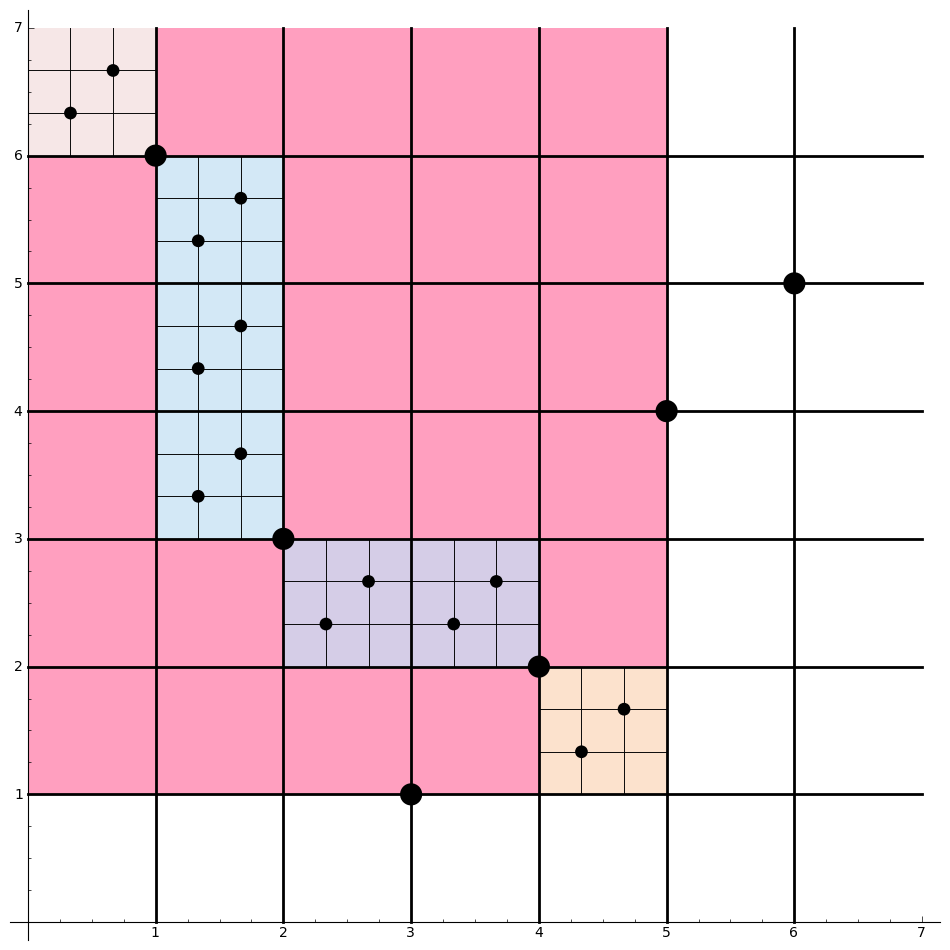
\includegraphics[scale=0.28]{mynstur}
                \caption{Einstaklega áhugavert}
            \label{fig:mynstur}
\end{figure}
            \end{center}
            \end{table}
        
\section{Myndir}
    Eins og lesa mátti í kafla \ref{sec:kafli2}, þá er um að gera að nýta sér Wiki-bókina til að komast að því hvernig maður setur myndir, eins og til dæmis Mynd \ref{fig:mynstur}, inn í skjalið.


\section{Jöfnur og formúlur}
    Jöfnur og stæður, eins og t.d. x eða x2 + 2 = 3, er hægt að rita inni í texta. Ef formúlur er langar, þá er hægt að setja þér í sér línu. Til dæmis er formúlan

        \[
        \sum_{i=1}^{10} 1cm(x_i,y')
        \]
frekar löng, og er sett í sér línu.

\section{Kóði}
    Við getum skrifað stutta kóðabúta inni í texta, eins og t.d. int x = 3 og reader(). Þar að auki getum við sett inn heilu C++ forritin, eins og Forrit ? sýnir.
    
\begin{center}
Forrit 1: Merkilegur kóði
\begin{lstlisting}[frame=single]
typedef int semaphore;
semaphore mutex1 = 1, mutex2 = 1, mutex3 = 1;
semaphore dbr = 1, dbw = 1;
int rc = 0, wc = 0;

void reader(void)
{
    while(true)
    {
        down(&mutex3);
        down(&dbr);
        down(&mutex1);
        rc += 1;
        if (rc == 1) down(&dbw);
        up(&mutex1);
        up(&dbr);
        up(&mutex3);

        readDatabase();

        down(&mutex1);
        rc -= 1;
        if (rc == 0) up(&dbw);
        up(&mutex1);
        useDataRead();
    }
}

\end{lstlisting} 
\end{center}

\section{Reiknirit}
    Til að finna stystu leið frá einum hnút, til allra hinna hnútanna í gefnu neti, er hægt að nota Reiknirit ?.

\end{document}
